\section{Approach}
\label{sec:approach}
\subsection{Formalization}
\label{sec:formalization}

Let $S$ be a set of stable bug fixing patches and $P$ a set of all bug fixing patches in Linux kernel. We call $U \in (S \cap P ) $ is a set of unknown bug fixing. In our problem, we try to provide a bug fixing patches ranking $\subset P^2$ for a developer, where each bug fixing patch has to meet the following properties~\cite{rendle2009bpr}:
\begin{itemize}
	\item \textit{Totality:} $\forall i,j \in P: i \neq j \Rightarrow (i > j) \vee (j > i)$
	\item \textit{Antisymmetry:} $\forall i,j \in P: (i > j) \wedge (j > i) \Rightarrow i = j$ 
	\item \textit{Transitivity:} $\forall i,j,k \in P: (i > j) \vee (j > k) \Rightarrow i > k$ 
\end{itemize}

\subsection{Bug Fixing Patch Ranking}
\label{sec:bugranking}
\begin{figure*}[t!]
	\centering
	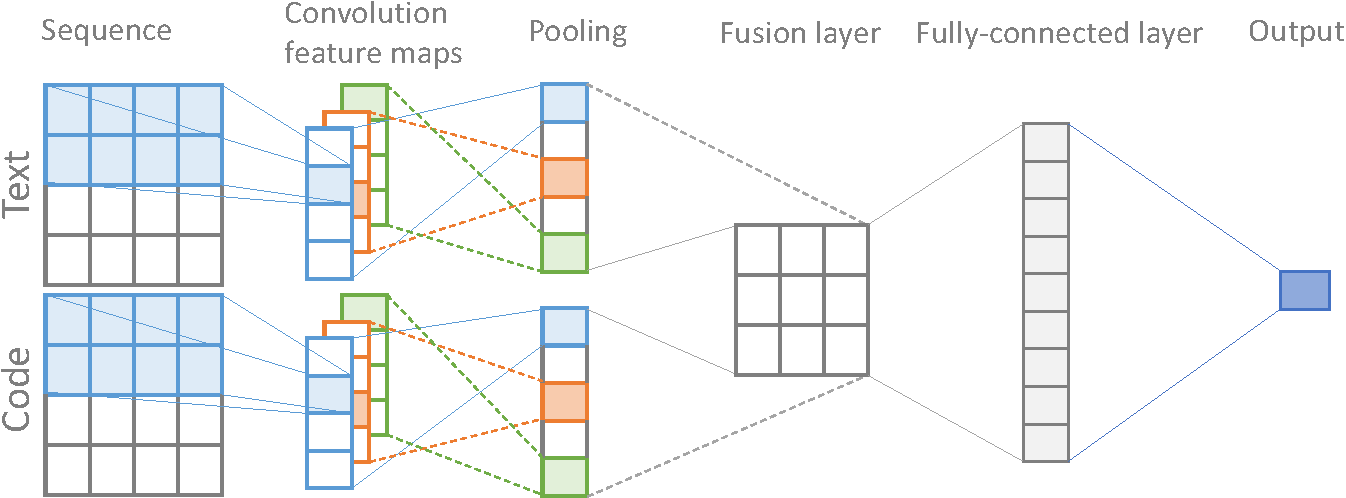
\includegraphics[width=1.0\textwidth]{BugPatchingRanking_v4-cropped.pdf}
	\caption{An architecture of bug fixing patches ranking model in Linux kernel.}
	\label{fig:bugranking}
\end{figure*}

The architecture of bug fixing patch ranking is represented in Fig.~\ref{fig:bugranking}. Our model based on convolutional neural network~\cite{lecun1995convolutional} to map bug fixing patches to vectors, which can be used to compute their ranking score. In the following, we describe how the model computes the ranking score given by a pair of bug fixing patches. We briefly explain each component (i.e., hidden layer, logistic function, etc.) of our model.

\subsection{Learning Relationship Between Text and Code in Single Patch}
\label{sec:learningTextandCode}
In Linux kernel, each patch contains both a textual commit message and commit code. The commit message, which can help a developer to speed up the reviewing process, is a short description of source code change. The commit code is the changes that are applied on the buggy file. 


\subsection{Hidden Layer}
\label{sec:hiddenlayer}

\subsection{Feature Representation}
\label{sec:feature}

\subsection{Output Layer}
\label{sec:output}

\subsection{Training}
\label{sec:trainingmodel}
Our model is trained by minimizing the cross-entropy lost function: 
\begin{equation}
\begin{split}
	\mathcal{L} &= -\text{log}\prod^\text{N}_{i \in S,j \in U}p(y_{ij}|p_i,p_j) + \lambda \lVert \theta \lVert^2_2 \\ &= -\sum_{i \in S,j \in U}^\text{N} \text{log } \sigma (\textbf{a}_{ij}) + \lambda \lVert \theta \lVert^2_2
\end{split}
\end{equation}
where $S$ and $U$ are the stable and unknown bug fixing patches datasets respectively, $y_{ij} = 1$ since $p_i$ has higher rank compared to $p_j$, N is the total number pairs of bug fixing patches in $S$ and $U$, $\sigma(.)$ represents the logistic function to identify the rank order of patches pair. $\text{\textbf{a}}_{ij}$ is the output of our ranking model and can be decomposed as:
\begin{equation}
\begin{split}
\text{\textbf{a}}_{ij} & = \text{\textbf{a}}_i - \text{\textbf{a}}_{j} \\
% & = \sigma (\text{\textbf{mean}}(\tilde{x}_{p_i}) - \text{\textbf{mean}}(\tilde{x}_{p_j}))
\end{split}
\end{equation}
to satisfy the properties mentioned in Sec.~\ref{sec:formalization}. 
%. $\tilde{x}_{p_i}$ and $\tilde{x}_{p_j}$ are the feature representations of two patches $p_i$ and $p_j$ respectively (see Fig.~\ref{fig:bugranking}). \textbf{mean}$(.)$ returns the mean of vector elements of each feature representation. 

\subsection{Regularization}
\label{sec:regularization}



